\section{Задача Мостов Шредингера}
\label{sec:Chapter1} \index{Chapter1}
Существует несколько эквивалентных задач мостов Шрёдингера. Для понимания проблематики актуальных решений и перед тем как перейти к постановки задачи и предложенному методу решения, потребуется рассмотреть их, а также итеративные алгоритмы решения данных задач. Для этого, сначала потребуется ввести определение меры пути.

\begin{definition}[Мера пути]
    Для процесса Ито вида 
    \begin{equation*}
        dx(t) = b(t) + \sigma(t)d\beta(t),
    \end{equation*}

    определенного на интервале $[0, T]$, с функция сноса -- $b(t)$, $\sigma(t)$ -- функция волатильности, $\mathbb{P}$ называется мерой пути данного процесса с пространством исходов $\Omega = C([0, T], \mathbb{R}^d)$, если распределение $\mathbb{P}$ описывает слабое решение данного стохастического дифференциального уравнения (СДУ).
\end{definition}

Иначе говоря, мера пути представляет собой меру вероятности, ассоциированную со случайным процессом, задаваемым СДУ. Например, $\mathbb{W}^\gamma$ является мерой Винера и представляет вероятность траекторий винеровского процесса с волатильностью $\sqrt{\gamma}$ то есть $dx(t) = \sqrt{\gamma}d\beta(t)$.

\subsection{Динамическая постановка задачи мостов Шрёдингера}
Задача мостов Шрёдингера возникает из вопроса: как ограничить некоторый заданный случайный процесс? Ответ дает теория больших отклонений, в частности, теорема Санова \cite{sanov}.

\begin{theorem}[Санов]
    Пусть заданы $\{x_i(t)\}^N_{i=1}\sim \mathbb{W}^\gamma$ -- независимые одинаково распределённые траектории из меры пути априорного винеревского процесса $\mathbb{W}^\gamma$, где $x_i (t) \in \mathcal{C}([0,T], \mathbb{R}^d), \forall i=\overline{1, N}$. Также пусть дана эмпирическая мера $\hat{\mathbb{W}}$ по заданным траекториям:
    \begin{equation*}
        \hat{\mathbb{W}}(A)=\frac{1}{N}\sum_{i=1}^N\mathds{1}\left(x_i(t)\in A\right), A\in \mathcal{B}(\mathbb{R}^d)^{[0,T]},
    \end{equation*}
    тогда вероятность, что $\hat{\mathbb{W}}$ ограничена заданными распределениями $\pi_0$ и $\pi_T$ задана следующей асимптотической оценкой:
    \begin{equation}
        P\left(\hat{\mathbb{W}} \in \mathcal{D}(\pi_0, \pi_T)\right) \xrightarrow{N\rightarrow \infty} \exp\left(-N\inf_{\mathbb{Q} \in \mathcal{D}(\pi_0, \pi_T)}D_{KL}\mathbb{(Q||W})\right),
        \label{eq:sanov-theorem}
    \end{equation}
    где $\mathcal{D}(\pi_0, \pi_T)$ -- множество всех мер путей ограниченных заданными распределениями $\pi_0$ и $\pi_T$.
\end{theorem}

Таким образом, для того, чтобы ограничить $\hat{\mathbb{W}}$ распределениями $\pi_0$ и $\pi_T$, необходимо:
\begin{equation*}
    P\left(\hat{\mathbb{W}} \in \mathcal{D}(\pi_0, \pi_T)\right) = 1,
\end{equation*}
следовательно, степень экспоненты должна быть нулевой. Для этого необходимо, чтобы дивергенция меры пути совпадали и Кульбака-Лейблера была нулевой.

Первой постановкой является динамическая. Она прямо следует из асимптотической оценки Санова \ref{eq:sanov-theorem} и находит такую меру пути $\mathbb{Q}$, ограниченную заданными распределениями $\pi_0(x)$ и $\pi_T(y)$, что наиболее близка с точки зрения теории информации к априорной мере пути винеровского процесса $\mathbb{W}^\gamma$ с волатильностью $\sqrt\gamma$:
\begin{equation}
    \hat{\mathbb{Q}} = \arg\min_{\mathbb{Q}\in \mathcal{D}(\pi_0, \pi_T)} D_{KL}\mathbb{(Q||W}^\gamma)
    \label{dyn}
\end{equation}

\subsection{Статическая постановка мостов Шрёдингера}
Помимо динамической постановки также существует и статическая. Для её вывода и доказательства эквивалентности рассмотрим декомпозицию дивергенции Кульбака-Лейблера в уравнении \ref{dyn}. Сначала выразим производную Радона-Никодима, условную по $\textbf{x}(0)=x$ и $\textbf{x}(T)=y$:
\begin{equation*}
    \frac{d\mathbb{Q}}{d\mathbb{W}^\gamma} = \frac{q(x, y)}{p^{\mathbb{W}^\gamma}(x, y)}\frac{d\mathbb{Q}_{(0,T)}}{d\mathbb{W}^\gamma_{(0,T)}}(\cdot|x,y)
\end{equation*}

Подставляя это выражение в дивергенцию Кульбака-Лейблера в уравнении \ref{dyn}, получаем:
\begin{equation*}
    \begin{split}
        D_{KL}\mathbb{(Q||W}^\gamma) = \mathbb{E_Q}\left[\log \frac{d\mathbb{Q}}{d\mathbb{W}^\gamma}\right] = \mathbb{E_Q}\left[\log \frac{q(x, y)}{p^{\mathbb{W}^\gamma}(x, y)}\frac{d\mathbb{Q}_{(0,T)}}{d\mathbb{W}^\gamma_{(0,T)}}(\cdot|x,y)\right] = \\ = \int\log \frac{q(x, y)}{p^{\mathbb{W}^\gamma}(x, y)} d\mathbb{Q} + \int\log \frac{d\mathbb{Q}_{(0,T)}}{d\mathbb{W}^\gamma_{(0,T)}}(\cdot|x,y)d\mathbb{Q}= \\ = \int q(x, y)\log \frac{q(x, y)}{p^{\mathbb{W}^\gamma}(x, y)} dxdy + \int\log q(x, y)\frac{d\mathbb{Q}_{(0,T)}}{d\mathbb{W}^\gamma_{(0,T)}}(\cdot|x,y)d\mathbb{Q}_{(0,T)} = \\ = D_{KL}\left(q(x, y) || p^{\mathbb{W}^\gamma}(x, y)\right) + \mathbb{E}_{q(x, y)}\left[D_{KL}\left(\mathbb{Q}_{(0,T)}(\cdot|x,y) || \mathbb{W}^\gamma_{(0,T)}(\cdot|x,y)\right)\right]
    \end{split}
\end{equation*}

Видно, что второй член дивергенции Кульбака-Лейблера не учитывает маргинальные распределения, поэтому он не влияет на оптимизационные ограничения и может быть отброшен. Таким образом, не рассматривается динамика на интервале $(0, 1)$ и для решения задачи важно только совместное распределение между крайними маргинальными распределениями. 

В результате получается статическая постановка задачи мостов Шрёдингера:
\begin{equation}
    \left\{ 
    \begin{array}{c}
        \hat q(x,y) = \arg\min_{q(x,y)} D_{KL}(q(x,y)||p^{\mathbb{W}^\gamma}(x,y)), \\
        \pi_0(x) = \int q(x,y)dy, \\
        \pi_T(y) = \int q(x,y)dx,
        \label{static}
    \end{array}\right.
\end{equation}
где $q(x,y)$ — это совместное распределение, которое является ближайшим к броуновскому движению при условии ограничений на маргинальные распределения. 

\subsection{Система Шрёдингера}
Третья формулировка требует рассмотрения лагранжиана статической постановки \ref{static}:
\begin{equation*}
    \begin{split}
        L(q, \lambda, \mu) = D_{KL}(q(x,y)||p^{\mathbb{W}^\gamma}(x,y)) + \int \lambda(x)\left(\int q(x, y)dy - \pi_0(x)\right)dx + \\ + \int \mu(y)\left(\int q(x, y)dy - \pi_T(y)\right)dy
    \end{split}
\end{equation*}

Предполагая, что $p^{\mathbb{W}^\gamma}(x,y) = p_0^{\mathbb{W}^\gamma}(x)p^{\mathbb{W}^\gamma}(y|x)$, где $p_0^{\mathbb{W}^\gamma}(x)$ может быть любым, а так как априорный процесс является винеровским, $p^{\mathbb{W}^\gamma}(y|x)=\mathcal{N}(y|x, \gamma I_d)$, приравняем $\frac{\partial L(q, \lambda, \mu)}{\partial q(x,y)}$ нулю и получим:
\begin{equation*}
    q^*(x, y) = \exp{(\ln{p^{\mathbb{W}^\gamma}(x,y)} - \lambda(x) - 1)}p^{\mathbb{W}^\gamma}(y|x)\exp{(-\mu(y))}
\end{equation*}

Теперь положив, что  $\hat\phi_0(x) = \exp{(\ln{p^{\mathbb{W}^\gamma}(x,y)} - \lambda(x) - 1)}$ и $\phi_T(y) = \exp{(-\mu(y))}$ получаем:
\begin{equation*}
    q^*(x, y) = \hat\phi_0(x)p^{\mathbb{W}^\gamma}(y|x)\phi_T(y),
\end{equation*}
удовлетворяющее:
\begin{equation*}
    \hat{\phi}_0(x) \int \phi_T(y) p_W^\gamma(y|x) dy = \pi_0(x),
\end{equation*}
\begin{equation*}
    \phi_T(y) \int \hat{\phi}_0(x) p_W^\gamma(y|x) dx = \pi_T(y),
\end{equation*}

Теперь переобозначим термины с интегралами как:
\begin{equation*}
    \phi_0(x) = \int \phi_T(y) p_W^\gamma(y|x) dy,
\end{equation*}
\begin{equation*}
    \hat{\phi}_T(y) = \int \hat{\phi}_0(x) p_W^\gamma(y|x) dx.
\end{equation*}

Объединяя все вместе, следующая линейная функциональная система является системой Шрёдингера:
\begin{equation}
    \left\{ 
    \begin{array}{c}
        \hat{\phi}_0(x) \phi_T(x) = \pi_0(x), \\
        \hat{\phi}_T(x) \phi_T(y) = \pi_T(y).
    \label{sys_sb}
    \end{array}\right.
\end{equation}

\subsection{Динамические полумосты Шрёдингера}
Наиболее важной для этой работы является постановка задачи полумостов Шрёдингера. В отличии от оригинальной задачи мостов Шрёдингера, задача полумостов ограничивается только на одну сторону, то есть $\mathcal{D}(\pi_0(x), \cdot)$ или $\mathcal{D}(\cdot, \pi_T(y))$. 

Более формально задача прямого полумоста, то есть, ограниченного в момент времени 0, определяется так:
\begin{equation}
    \mathbb{Q}^*=\arg\min_{\mathbb{Q}\in\mathcal{D}(\pi_0(x), \cdot)}D_{KL}\left(\mathbb{Q}||\mathbb{W}^\gamma\right),
    \label{eq:forward_hsb}
\end{equation}
а задача обратного определятся следующим образом:
\begin{equation}
    \mathbb{P}^*=\arg\min_{\mathbb{P}\in\mathcal{D}(\cdot, \pi_T(y))}D_{KL}\left(\mathbb{P}||\mathbb{W}^\gamma\right)
    \label{eq:backward_hsb}
\end{equation}

В отличии от оригинальной постановки задачи мостов Шрёдингера, задачи обоих полумостов имеет следующее аналитическое решение:
\begin{equation*}
    \mathbb{Q}^*(A_0\times A_{(0,1]})=\int_{A_0\times A_{(0,1]}}\frac{d\pi_0}{p_0^{\mathbb{W}^\gamma}}(x)d\mathbb{W}^\gamma
\end{equation*}
\begin{equation*}
    \mathbb{P}^*(A_{[0,T)} \times A_T)=\int_{A_{[0,T)} \times A_T}\frac{d\pi_T}{p_T^{\mathbb{W}^\gamma}}(y)d\mathbb{W}^\gamma,
\end{equation*}
для прямого и обратного мостов соответственно.

\subsubsection{Статические полумосты Шрёдингера}
Аналогично и оригинальной постановке рассмотрим статическую формулировку полумостов. Прямой полумост задается следующим образом:
\begin{equation}
    \begin{split}
        q^*(x,y)=\arg\min_{q(x,y)\in\mathcal{D}(\pi_0(x), \cdot)}D_{KL}\left(q(x,y)||p^{\mathbb{W}^\gamma}(x,y)\right), \\
        \text{такое, что } \pi_0(x) = \int q(x, y)dy,
    \end{split}
\end{equation}
а обратный:
\begin{equation}
\begin{split}
    p^*(x,y)=\arg\min_{p(x,y)\in\mathcal{D}(\cdot, \pi_T(y))}D_{KL}\left(p(x,y)||p^{\mathbb{W}^\gamma}(x,y)\right), \\
    \text{такое, что } \pi_T(y) = \int q(x, y)dx.
\end{split}
\end{equation}

Как и для динамической постановки статическая обладает аналитическим решением:
\begin{equation*}
    q(x,y)^*=p(x,y)^{\mathbb{W}^\gamma}\frac{\pi_0(x)}{p^{\mathbb{W}^\gamma}(x)},
\end{equation*}
\begin{equation*}
    p(x,y)^*=p(x,y)^{\mathbb{W}^\gamma}\frac{\pi_T(y)}{p^{\mathbb{W}^\gamma}(y)},
\end{equation*}
для прямого и обратного полумостов, соответственно.

Полумосты полезны не только из-за того, что обладают аналитическим решением, но и тем, что позволяют легко справится с ограничением на искомый мост, заменяя его на задачу с начальным значением. Также благодаря полумостам итеративною решается оригинальная задача мостов Шрёдингера.

\subsection{Методы решения мостов Шрёдингера}
Далее рассмотрим итеративные алгоритмы, которые решаяют задачу мостов Шрёдингера.

Алгоритм Фортета \ref{alg:fortret} является одним из старейших методов, доказавших свою сходимость для решения системы Шрёдингера. Этот алгоритм, впервые предложенный Фортетом в 1940 году \cite{fortret}, включает итеративный процесс, обеспечивающий выполнение маргинальных условий системы Шрёдингера \ref{sys_sb} для распределений в моменты времени $t=0$ и $t=T$.

\begin{algorithm}
\caption{Фортет}\label{alg:fortret}
\KwInput{$\pi_0(x)$, $\pi_T(y)$, $p(y|x)$}
\KwOutput{$\hat\phi^{(i)}_0(x)$, $\phi^{(i)}_T(y)$}
Инициализируем $\phi_0^{(0)}(x)$ такое, что $\phi_0^{(0)}(x)<<\pi_0(x)$\;
Инициализируем $i = 0$\;
\While{не сойдется}{
    $\hat\phi_0^{(i)}(x):=\frac{\pi_0(x)}{\phi_0^{(i)}(x)}$\;
   $\hat\phi_T^{(i)}(y):=\int p(y|x)\hat\phi_0^{(i)}(x)dx$\;
    $\phi_T^{(i)}(y):=\frac{\pi_T(y)}{\hat\phi_T^{(i)}(y)}$\;
    $\hat\phi_T^{(i+1)}(x):=\int p(y|x)\phi_T^{(i)}(y)dy$\;
    $i:=i+1$\;
   }
\end{algorithm}

Алгоритм Фортета фактически чередует выполнение маргинальных условий для моментов времени $t=0$ и $t=T$, пока не сойдется. В результате достигается решение, соответствующее заданным граничным условиям для обоих моментов времени.

Другим методом решения задачи мостов Шрёдингера является алгоритм Iterative Proportional Fitting (IPF). IPF -- это метод, используемый для нахождения дискретное совместное распределение при заданных маргинальных, используя принципы максимальной энтропии. Однако в контексте мостов Шрёдингера, а именно статической постановки задачи, в 1968 году Кульбаком \cite{kullback} был разработан непрерывный вариант IPF, а сходимость его доказана Рушендорфом \cite{kullback-prove}.

\begin{algorithm}
\caption{IPF}\label{alg:ipfp}
\KwInput{$\pi_0(x)$, $\pi_T(y)$, $p(y|x)$}
\KwOutput{$q_i^*(x, y), p_i^*(x, y)$}
Инициализируем $p_T^{\mathbb{W^\gamma}}(y)$ такое, что $p_T^{\mathbb{W^\gamma}}(y)<<\pi_T(y)$\;
Инициализируем $q_0^*(x,y) := p^{\mathbb{W}^\gamma}(x,y)$\;
Инициализируем $i = 0$\;
\While{не сойдется}{
    $p_i^*(x,y) = \arg\min_{p(x,y)\in \mathcal{D}(\cdot, \pi_T(y))}D_{KL}(p(x,y)||q^*_{i-1}(x,y))$\;
    $q_i^*(x,y) = \arg\min_{q(x,y)\in \mathcal{D}(\pi_0(x), \cdot)}D_{KL}(q(x,y)||p^*_i(x,y))$\;
    $i:=i+1$\;
   }
\end{algorithm}

\begin{figure}
    \centering
    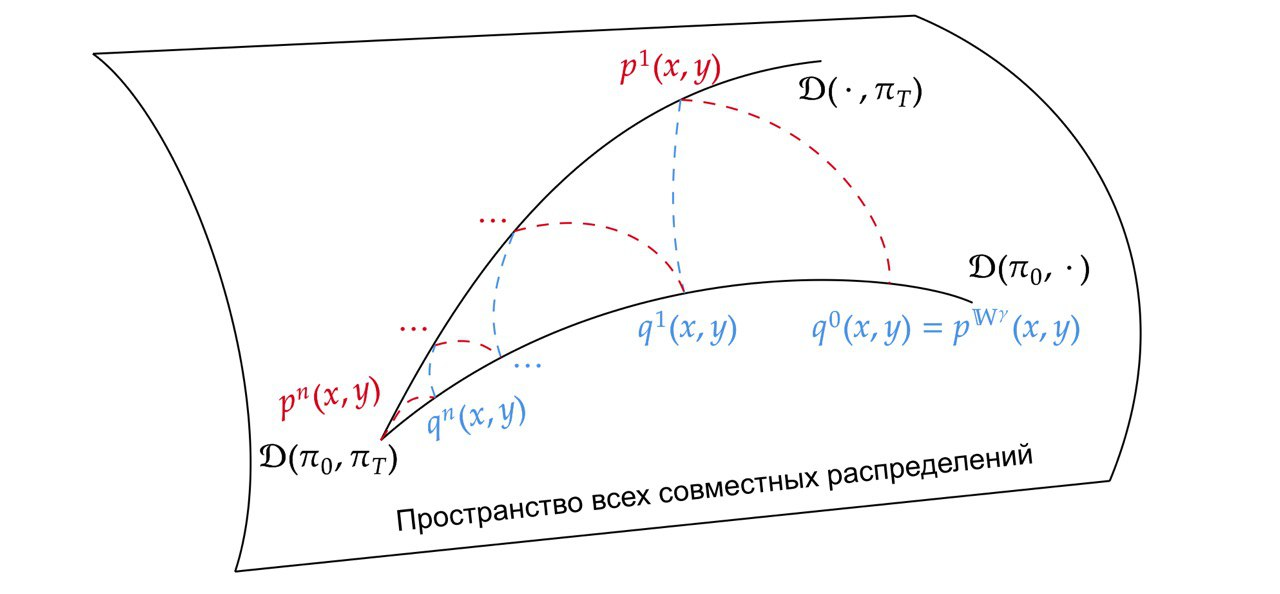
\includegraphics[width=1\linewidth]{images/ipfp.png}
    \caption{Иллюстрация алгоритма IPF}
    \label{fig:ipfp}
\end{figure}

Суть алгоритма Кульбака заключается в чередовании решения полумостов начиная с обратного. Можно заметить, что если шаги 5 и 6 переписать с помощью аналитического решения задачи полумостов, а также начать алгоритм с прямого прохода, данный алгоритм сводится к алгоритму Фортета. Иллюстрация IPFP изображена на рисунке \ref{fig:ipfp}

Следующий алгоритм generalised IPF (g-IPF) обобщает IPF, предложенный Кульбаком, применяя его к динамической постановке задачи. Этот метод идентичен обычному IPF, однако на каждом шаге минимизируется дивергенция Кульбака-Лейблера между двумя мерами путей. 
\newpage
\begin{algorithm}
\caption{g-IPF}\label{alg:g-ipfp}
\KwInput{$\pi_0(x)$, $\pi_T(y)$, $\mathbb{W}^\gamma$}
\KwOutput{$\mathbb{Q}_i^*(x, y), \mathbb{P}_i^*(x, y)$}
Инициализируем $\mathbb{Q}_0^*(x,y) := \mathbb{W}^\gamma$\;
Инициализируем $i = 0$\;

\While{не сойдется}{
    $\mathbb{P}_i^*(x,y) = \arg\min_{\mathbb{P}(x,y)\in \mathcal{D}(\cdot, \pi_T(y))}D_{KL}(\mathbb{P}(x,y)||\mathbb{Q}^*_{i-1}(x,y))$\;
    $\mathbb{Q}_i^*(x,y) = \arg\min_{\mathbb{Q}(x,y)\in \mathcal{D}(\pi_0(x), \cdot)}D_{KL}(\mathbb{Q}(x,y)||\mathbb{P}^*_i(x,y))$\;
    $i:=i+1$\;
   }
\end{algorithm}

\newpage